\chapter{Technologies} \label{ch:technologies}

\section{Docker}
When discussing containers, Docker cannot be left out of the discussion. Docker is an open-source platform designed to automate the creation, deployment, scaling and management of containerized applications. It is, by far, the most widely adopted tool for containerization. Docker allows the packaging of applications and their dependencies into lightweight and easily portable containers that can be deployed consistently across a wide range of environments. This portability ensures that applications behave identically, whether running on a developer's laptop, a staging environment, or a production server. To provision containers, Docker uses images. Docker images are read-only templates used to create containers, similar to .iso files for virtual machines, but are more lightweight and versatile. Docker images bundle everything an application needs to run, including the operating system, application code, dependencies, libraries, and configuration metadata. The metadata often includes the entrypoint script, a set of commands executed when the container is instantiated. An important feature of Docker images is their layered architecture. Each layer represents a distinct change, such as adding a file, installing a package, or modifying a configuration. This layered design allows developers to build images on top of existing ones, significantly reducing build times, image sizes, and data transfer requirements. The runtime environment responsible for building, running, and managing containers is the Docker Engine, and it consists of three main components. The first is the Docker Daemon, a background service responsible for managing Docker objects, such as containers, images, volumes, and networks. Next is the Docker Command-Line Interface (CLI), which provides a way to interact with Docker through terminal commands. Finally, the REST API enables programmatic access to Docker's functionalities. Docker images are created using Dockerfiles, which act as blueprints for the image creation process. A Dockerfile contains step-by-step instructions for building an image, including the base image, commands to configure the environment, install dependencies, and metadata such as port configurations and  the entrypoint script. This declarative approach ensures reproducibility, as anyone with the Dockerfile can recreate the same image, ensuring consistency across teams. Since images are meant to be portable and used over multiple environments, remote registries to store and fetch images from are crucial. Docker Hub is a free, widely used registry provided by the wider Docker ecosystem. Hand in hand with containers, Docker enables the creation and management of other resources critical for smooth operation. Volumes are a mechanism for persisting data generated and used by containers. Unlike ephemeral container storage, volumes ensure data remains intact even after container deletion. Docker also creates networks, enabling container interconnectivity, and  communication between containers and the outside world. For handling deployments of multiple containers in a programmatic way, Docker Compose can be utilized. Docker Compose is a tool that utilizes simple YAML files to manage multi-container deployments or applications, by defining services, networks, and volumes required. This approach reduces complexity and enhances reproducibility, making it easier to manage applications with multiple interconnected components. Finally, Docker provides a native container orchestration platform, Docker Swarm, but on a production level it is outclassed by other, more robust and feature-rich solutions, such as bare-metal Kubernetes or cloud Kubernetes services like Amazon Elastic Kubernetes Service (EKS) and Google Kubernetes Engine (GKE) that offer seamless integration and scalability.\cite{containers_docker}


\begin{figure}[!h]
    \graphicspath{ {./diagrams/} }
    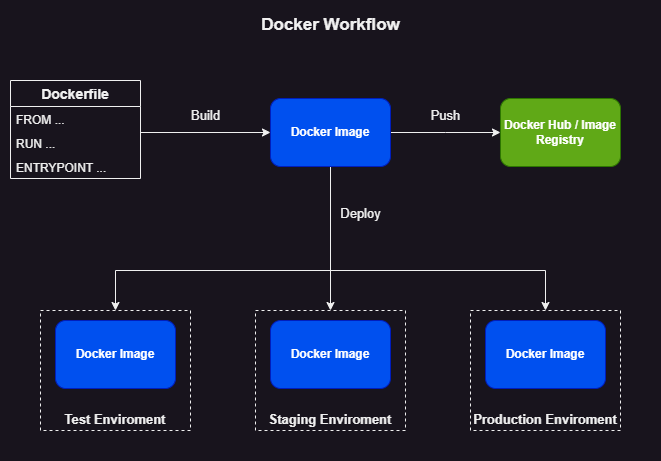
\includegraphics[scale=0.48]{docker_wf.png}
    \centering
    \caption{Docker Workflow}
    \label{fig:docker_wf}
\end{figure}

\section{Prometheus}

\section{Grafana}

\section{MQTT}